\chapter{Configuration Management}
\label{chap:configuration-management}
\index{Configuration Management}

\begin{quote}
{\em The entropy of an isolated system never decreases.} \\
-- {Second Law of Thermodynamics}
\end{quote}

% XXX need graphic here

\section{Introduction}
\label{configuration-management:introduction}

As much as we would like them to be, computer systems
are not static: files are created, modified, or
removed; users log in and run commands; services are
started or terminated.  In addition, the requirements
of the systems, dictated at least in part by evolving
business needs or emerging technologies are changing
all too frequently as well.  This leads to new
software being added, patched or upgraded; user
accounts are added or removed; jobs are scheduled or
their frequency changed; interactions with other
systems are enabled or prevented.  In other words, our
systems do continuously undergo change.

On a single host, such changes are made by local
modification of system configuration files, invocation
of specific commands, and the installation or tuning
of different applications.  As we configure our
machines, we may create detailed documentation about
how to set up a given service, and the more systems we
have, the more often we have to repeat the same steps
to configure them, to upgrade software, or to rebuild
them when they inevitably fail.  Updating
documentation to reflect the changes we may have made
after the latest software update is tedious and error
prone -- it would be much easier to initially identify
the changes, document them, and then have them be
applied so that our hosts' configuration reflects the
documentation, not the other way around.

Taking this approach even further, we begin to build
not only a document outlining what commands to
execute, but a central inventory of what hosts perform
which functions, which services are running and which
software needs to be installed to produce, for
example, a running web server suitable for serving
production traffic.

We rarely operate on a single host only, and the
larger our infrastructure, the more important it
becomes to be able to discover systems by their
attributes.  For example: in order to apply a security
update to our web servers, we need to first know
exactly which of our many hosts are running the
vulnerable version, and then perform the same steps of
upgrading the service on them.  Since we cannot
possibly keep track of hundreds of changes across
thousands of systems ourselves, we delegate the task
of applying well defined sets of changes to (possibly
very large) numbers of systems to a class of software
known as \gls{scm-cm}\index{Configuration Management}
systems, or ``CMs''.

We have hinted at the capabilities of such solutions
before: near the end of Chapter
\ref{chap:software-installation}, we explained that by
the time the OS is installed on a host, we already
have to perform at least a minimal amount of custom
configuration.  We also noted that in order to be able
to add software on a host, CM requires a tight
integration with the system's package manager.

Following that, we discussed user accounts in the
previous chapter, another example of our system's
changing characteristics: the set of users that should
be allowed access to a given host changes regularly
and frequently as people join or leave the
organization.\footnote{Depending on the size of the
organization, this data needs to be tightly integrated
with a larger staff directory as well as various other
systems such as payroll, your benefits related
databases, or perhaps an external index of who should
get keycards for the offices.  Integration of these
services, many of which are nowadays outsourced to
third party providers, is well beyond the scope of
this chapter, however.  Once again, we're scratching
the surface of additional complex topics.} Regardless
of whether you use an \gls{ldap}\index{LDAP} or Active
Directory (AD) service or whether you push changes to
each hosts' {\tt /etc/passwd} file, certain
modifications are necessary on each server.  

It is the ironic fate of many a system administrator
to have, at one time or another, written a set of
programs to allow changes to all of their machines.
These programs tend to start out as simple shell
scripts that loop over all hostnames in the inventory,
using {\tt ssh(1)} and {\tt rsync(1)} to copy files
from one host to many, but as the environment grows,
the painful realization that this approach does not
scale starts to set in.  We begin to understand that
configuration management is not only about shuffling
files around, but it tracks and enforces {\em state}
on a system.  We also need to be able to control
running services and react to changes in the
environment.

Fortunately, a number of mature and flexible CM
solutions have emerged over the last few years.
Today's junior system administrators are already
likely to start out using tools like {\em
CFEngine}\cite{configuration-management:burgess:cfengine},
{\em
Chef}\cite{configuration-management:nelson-smith:chef},
{\em
Puppet}\cite{configuration-management:turnbull:pro-puppet},
or {\em
Ansible}\cite{configuration-management:ansible} to
automate configuration changes across both small and
large sets of hosts.  But even the most advanced
solution requires a fair amount of customization to be
integrated into your environment as you scale up, and
you will almost certainly learn valuable lessons as
you try to avoid writing your own CM system.

Being able to fully take advantage of configuration
management requires, not surprisingly, an initial
learning curve as well as some careful consideration
of how to organize and categorize your data as well as
your physical assets.  In this chapter, we will take a
look at how best to do this.  We will discuss the
principles on which configuration management systems
operate, as well as the significant benefits they
provide.

While reading this chapter, it may be useful to
remember the Second Law of Thermodynamics, quoted at
the beginning: our systems are in fact constantly
approaching an increased state of disorder.  Let us
find out, how configuration management systems can
counter this effect and help to restore order...

\begin{sidenote} {\bf Danger! Acronym Overload!} \\

The acronym {\em \glslink{scm}{SCM}} may also be used
for {\em Source Control Management}\index{Source
Control Management}, i.e. the tracking of code changes
in a repository.  Since we are talking entirely
about {\em Software} Configuration Management, and in
an attempt to minimize confusion, we will use the
acronym {\em CM} for both the terms ``configuration
management'' as well as ``configuration management
systems'' throughout this book.  When talking about
revision control\index{revision control}, we will use
the acronym \acrshort{vcs}\index{VCS} (for Version
Control System).  Admittedly, it doesn't help that
often times our CM files are stored in a VCS such as
\glslink{cvs}{CVS}...  \end{sidenote}


\section{Services, not Single Points of Failure}
\label{configuration-management:services-not-spofs}

In many large environments, it used to be common to
find at least one or two ancient systems that system
administrators were afraid to touch.  Often these
servers provided a number of critical services, and
their configuration was as equal parts custom scripts,
undocumented dependencies, combined with some black
magic.  Making {\em any} change on such a system
required tribal knowledge, manual editing of
configuration files, could wreak havoc, and cause
significant downtime.

You still find symptoms of this approach to system
administration in many organizations, but -- necessity
being the mother of invention -- most organizations
nowadays have found ways to make their services
slightly more resilient (although certainly no less
complex).  ``Cattle, not pets'' is a common phrase
expressing this shift in mindset:  instead of grooming
and coddling individual systems, we should regard any
one server as replacable, easy to tear down and
recreate on a moment's notice.  Instead of focusing on
any individual host, we now begin by defining a {\em
service}, identifying its requirements and then
applying the required changes to any suitable hardware
system.  What used to be a unique, fragile, \gls{spof}
becomes a flexible, easily repeatable process to
recreate the functionality provided by any given host.

Consider the example of a single server providing
authentication services to your organization.  Since
it is such a crucial component of the infrastructure,
carefully maintained with custom scripts developed
over the years we may be averse to changing anything
on the host so as not to impact the reliability of the
service it provides.

We may provide added availability by installing a
failover instance or using a fault-tolerant protocol
allowing communication with multiple such hosts, but
downtime is eventually unavoidable, and hardware
failure may strike at any time.  Rebuilding such
special ``snowflake'' systems -- a term often used to
convey both their uniqueness and fragility -- is
painful and time consuming.  On the other hand, if we
have a well-defined procedure to build an
authentication server, we can easily replace it at
any time with minimal effort.\footnote{Experience has
shown us that {\em any} process that carries increased
risk ought to be automated and performed {\em
frequently}.  This may initially seem paradoxical, as
our insticts tell us to avoid risk.  However, the less
frequently we perform a given task, the more likely we
are to make mistakes; on the flip side, the more often
we perform it, the more likely we are to develop a
routine, to automate the task to be completed
unattended, a non-event.  This is a critically
important point, which we will repeat in Chapter
\ref{chap:automation}.} \\

Shifting your perception away from {\em host} to {\em
service} management allows you to abstract
requirements and define behaviour in a scalable
manner.  This way, fault tolerance improves, since in
case of an emergency another host can quickly be
bootstrapped into providing the given service in a
short amount of time.  Hosts become expendable rather
than individual, irreplaceable components, that can be
put into (or out of) production use through other
automated means.  Advanced systems that combine system
deployment, configuration management and service
monitoring react to fluctuations in traffic demands or
individual components' uptime by shifting traffic to
and from these parts, or they may possibly initiate
the instantiation of additional service nodes.  This
process is sometimes referred to as ``Service
Orchestration\index{Service Orchestration}'' (more on
that in Section
\ref{sec:missing:service-orchestration});
configuration management is an integral part of such
larger system.

\section{Defining Services and Requirements}
\label{configuration-management:defining-services}

System administrators tend to be very practically
oriented and are likely to start out setting up a new
service by installing the required software to
evaluate, tune it, change it, adapt it to the needs of
the environment and in this fashion end up with a
functional server.  If we wish to document this
process, so as to allow us to repeat it in the future
or possibly to automate it altogether, it is necessary
to trace back the decisions made in the process,
identify the changes made to the software and its
configuration files and codify all of this in a
repeatable manner.

This takes discipline and practice.  Documenting the
steps taken, as discussed in Section
\ref{documentation:types:processes}, is a good start.
We often are able to use this documentation as both a
way to double-check our process as well as a template
from which to derive instructions for our
configuration management system.  The tricky part is
making explicit the various assumptions we make about
the capabilities of the server on which the service is
to run.  Let us consider a few examples.

\subsection{Example Service: Syslog}
\label{configuration-management:defining-services:syslog}
\index{Syslog, Example Service Definition of}

To illustrate how a service might be defined, let us
walk through a simple, yet common example:  every
organization needs a way to collate, correlate and
monitor all sorts of different events, a topic we will
discuss in more detail in Chapter
\ref{chap:monitoring}.  A common solution involves the
use of a central {\tt loghost}, running the ubiquitous
\manpage{syslogd(8)} d\ae mon or perhaps one of its more
modern variants , such as the {\tt syslog-ng} or {\tt
rsyslog} software.

In its simplest setup, the d\ae mon accepts incoming
messages over the network via UDP port 514 and writes
them to local files with different permissions or
ownerships, based on its configuration.  In order to
be able to accomodate the high volume of messages
typically seen by a syslog server, the OS may require
a larger network buffer queue than the other systems
in the environment.  Finally, all the data needs to be
stored somewhere, so we require a large file system to
be mounted and log files to be periodically compressed
and archived.

Using these high-level requirements, we can identify a
few configuration steps necessary for this service
that may then get translated into a service definition
in the CM system's {\em \gls{dsl}}\index{DSL}.  As
an example, a {\em Puppet}\index{Puppet} ``manifest''
for the {\em syslog} service might look as shown in
Listing \ref{code:cm:syslog}.  This description of
requirements is of course non-exhaustive, but it
suffices to illustrate the general approach we would
like to take: all we need is to let the CM system --
{\em puppet}, in this case -- take these steps and
translate them into the commands to execute on the
target host.  With that in place, we can easily and
reliably bring up a new host to perform the
``syslog'' service.\footnote{Note that all of these
steps are by and large independent of the particular
Unix flavor the CM runs on.  By abstracting the
individual steps, such as the installation of a
package from their implementation (i.e. {\em how} to
invoke the package manager), we gain the flexibility
to repeat this as needed in different environments.}

\begin{minipage}{.9\linewidth}
\begin{lstlisting}[basicstyle=\scriptsize,label=code:cm:syslog,caption={Excerpt of a Puppet
``manifest'' defining the 'syslog' service.}]
class syslog {
  include cron
  include logrotate

  package {
    'syslog-ng':
      ensure  => latest,
      require => Service['syslog-ng'];
  }

  service {
    'syslog-ng':
      ensure  => running,
      enable  => true;
  }

  file {
    '/etc/syslog-ng/syslog-ng.conf':
      ensure  => file,
      source  => 'puppet:///syslog/syslog-ng.conf',
      mode    => '0644',
      owner   => 'root',
      group   => 'root',
      require => Package['syslog-ng'],
      notify  => Service['syslog-ng'];

    '/etc/logrotate.d/syslog-ng':
      ensure  => file,
      source  => 'puppet:///syslog/logrotate-syslog-ng',
      mode    => '0644',
      owner   => 'root',
      group   => 'root',
      require => Package['logrotate'];
  }
}
\end{lstlisting}
\end{minipage}

\subsection{Example Requirements: LDAP Client Configuration}
\label{configuration-management:defining-services:ldap-client}
\index{LDAP}

Our ``syslog'' example illustrated the definition of a
single service.  Despite our efforts to make this
service easy to replicate, we anticipate only a small
number of servers to be providing this service.  On
the other hand, we can also identify requirements that
will be applicable to a very large set of hosts, quite
possibly to every single host in our environment.

Let us consider the use case of account management in
an environment using a central \gls{ldap} directory.  We
need to ensure that every host is configured to
authenticate local access against the central service.
Our high-level configuration steps include the
installation of the LDAP client package, changes to
the authentication module's configuration file to
accept (and require) LDAP authentication, and a
configuration file pointing to the central LDAP
server.  Listing \ref{code:cm:ldap} illustrates the
translation of these steps into a {\em Chef}
``recipe''.

As before, all of these steps apply to all different
operating systems or OS flavors.  What is different
about this example is that it may well apply to other
hosts, including the previous {\em syslog} example.
It is useful to identify each of the specific cases
and define them independently instead of trying to
create monolithic definitions for every single host.
In particular, we often define a ``base''
configuration for all of our systems, including
default packages, security settings, authentication
methods and the like; individual service definitions
depend on this base configuration and bring in new
requirements applied to only those hosts providing the
given service.

That is, system and service definitions are {\em
additive}, and configuration management systems
determine and apply the appropriate final union of
settings needed for any combination. \\


\begin{minipage}{.9\linewidth}
\begin{lstlisting}[basicstyle=\scriptsize,label=code:cm:ldap,caption={[Excerpt
of an LDAP client authentication Chef
``recipe'']Excerpt of a Chef ``recipe'' defining LDAP
client authentication configuration. Note the
conceptual similarities to the Puppet DSL shown
earlier.}]
package "ldap-utils" do
  action :upgrade
end

template "/etc/ldap.conf" do
  source "ldap.conf.erb"
  mode   00644
  owner  "root"
  group  "root"
end

%w{ account auth password session }.each do |pam|
  cookbook_file "/etc/pam.d/common-#{pam}" do
    source   "common-#{pam}"
    mode     00644
    owner    "root"
    group    "root"
    notifies :restart, resources(:service => "ssh"), :delayed
  end
end
\end{lstlisting}
\end{minipage}

\subsection{CM Requirements}
\label{configuration-management:defining-services:requirements}

Different CM systems allow you to specify your service
requirements in different ways.  Due to their
particular evolution,  choice of programming language,
and internal architecture, they differ
significantly in detail, but exhibit conceptual
similarities.  Effectively, each CM system uses its
own \gls{dsl}, and you will have to get used to the
proper syntax to express your requirements.

Looking at the previous two examples, we can identify
some required concepts in configuration management
systems.  Generally speaking, the following (OS
agnostic) capabilities are required:

\subsubsection*{Software Installation}
The CM needs to be able to install software on the
hosts it manages.  More specifically, it needs to be
able to assure that software of a given version is
installed (or perhaps {\em not} installed).  It does
not need to duplicate the capabilities of the package
management system -- rather, it relies on the package
manager as a tool to accomplish the desired result.

The system administrator provides a definition of
which packages need to be present on the system,
optionally specifying the exact version or perhaps
simply requesting the ``latest'' available version.
In order to accomplish this, the CM needs to have
support for the package manager in use on the target
system.

However, as we discussed in Chapter
\ref{chap:software-installation}, it is important to
avoid introducing conflicts if you allow the CM to
install the ``latest'' version of a package, possibly
introducing a non-backwards compatible change -- keep
your configuration files in sync with the software
version they target!

\subsection*{Service Management}
\index{Service Management}

The CM needs to be able to define which software
services are supposed to be running on a given host.
A machine functioning as a web server, for example,
had better be running an HTTP d\ae mon.  In order for
some configuration changes to take effect, this d\ae
mon may need to be restarted, and in order to make
certain other changes, one may need to (temporarily)
shut down a service.

As starting, stopping, restarting and generally {\em
supervising} running processes is both software- and
OS dependent, the CM may fall back on the package
manager or system provided service management
mechanisms, such as {\tt /etc/rc.d} or {\tt
/etc/init.d} scripts, as well as more modern
frameworks such as Solaris's ``Service Management
Facility'' or Mac OS X's \manpage{launchd(8)}.

Coordinating service restarts across multiple systems
may require additional capabilities or settings within
the CM systems.  As noted above, CM may develop or
integrate with more formal service orchestration
functionality across a larger infrastructure.


\subsubsection*{File Permissions and Ownerships} The
CM needs to be able to set file permissions and
ownerships.  If these are not explicitly defined for a
given resource, then most systems will simply use the
OS defaults.  In the Unix world, this means falling
back on the default {\em umask}\index{umask} for
permissions and inheritance of ownership from the
parent directory via standard Unix semantics.

It is worth noting that asserting file ownerships has
additional implications: the user- and/or group-ID of
the given file owner need to be present on the
system.  Some CMs allow you to also manage user
accounts (they may add or remove users), while other
systems merely assert the existence of a given account
and produce an error if a specified file owner is not
present on the host in question.

That is, user management by itself may be performed by
the CM directly (that is, the CM systems adds or
removes users, adjust their account settings, creates
home directories etc.), or it may be handled via a
central account management system which the CM system
configures the host for.  Listing \ref{code:cm:ldap}
illustrates the latter case: Chef configures the host
to use LDAP for account management, and does not
further concern itself with account creation.

In addition, the distinction between ``regular'' user
accounts and service accounts -- see Chapter
\ref{multi-user:types} -- may further play a role
here: a central authentication service such as LDAP
may only provide information about ``regular'' users,
and system accounts not included in the base OS may be
added by e.g. the package manager.  As you can tell,
the interactions between all these systems is becoming
quite complex.

\subsubsection*{Installation of static files}
The CM needs to be able to install a given, static
file on all hosts.  This is an obvious requirement:
the management of local files lies at the heart of
every CM system, but it is worth identifying a few
distinct use cases.  Here, we provide a single file
that will be identical across all systems.  For
example, let us assume that you wish to provide a list
of SSH host keys as a system-wide {\tt known\_hosts}
entries under {\tt /etc/ssh/ssh\_known\_hosts}.  The
contents of this file will be the same across all of
your individual systems.

The CM system ensures that this file will be installed
-- as provided, with no further modifications -- on
the hosts.  If any local modifications were made since
the last time the CM ran, those will be overwritten.

The ability to modify an existing file on the target
system may seem like an important requirement for any
CM, as this is how we configure our systems manually.
However, this approach carries significant complexity:
For many different configuration files, it requires an
understanding of that file's syntax, and the risk of
conflicts introduced by letting local modifications
remain in place.  

With our strong preference of simpler solutions over
more complex ones, it is a better approach to let the
CM completely ``own'' all the files it manages.  That
is, define the contents of a file as derived from the
target system's properties (such as hostname, network
segment, etc.) and generate a new, static file in a
central place.

\subsubsection*{Generation of host-specific data}

The CM needs to be able to install host-specific
files.  For example, you may have different DNS or
Syslog servers available to your servers based on the
subnet they are deployed in.  Or you may wish to add
some information determined at runtime on the system
itself. For example, you might want to include the
current \manpage{uptime(1)} in the file
\manpage{/etc/motd}.

That is, some of the changes to a given file can be
determined in advance by the software, as in the case
of the DNS server setting: by knowing the IP address
of the host, you know which DNS server to write to
\manpage{/etc/resolv.conf}.  Other changes cannot be
known in advance: unless you are logged in on the
server in question, you can't well know the uptime it
would report.

To allow the system administrator to define dynamic
files with variable sections and actions, the CM needs
to provide a templating language as well as a means of
expanding these templates either prior to deployment
based on certain properties of the host (e.g. the
subnet it will reside on) or at execution time on the
system itself.

Some systems allow the use of a general purpose
programming language in building these templates.
This has the advantage of being able to provide great
flexibility in data generation.  On the other hand, it
also opens up room for unneeded complexity and may
reduce the readability or maintainability of the
templates.  The use of a \gls{dsl} can help avoid
common pitfalls and stir the user into the best
direction to solve a given problem.  ``Constraints are
friends.''\cite{configuration-management:brooks-design}
\index[names]{Brooks Jr., Frederick P.}

As a general rule of thumb, it is desirable to have
these templates be applied and the resulting files be
generated centrally, rather than on the hosts
themselves.  It is easy to assume that a CM needs to
execute within a host's context in order to take into
account that particular system's full state to apply
the correct settings.  However, when managing more
than just a few hundred hosts it actually becomes
reasonable (and less error prone!) to have
configuration management dictate the state on the
host {\em completely}.  While this requires the CM to
have full knowledge of a lot of the target systems'
state, this reduces the probability of any errors or
unpredicted events interfering with or changing the
state of the host, yielding undesired results.

Nevertheless, it remains a core requirement to be able
to generate a host-specific configuration file on the
target system, which is why all CM systems do provide
this functionality.  See Listing
\ref{code:cm:cfengine:dynamic-restart} for an example
of a change description that dynamically expands a
template on the host in question, conditionally
restarting the given service if (and only if!) the
resulting file was modified.

% XXX sshd_config.tmpl include?

\begin{figure}[!t]
\begin{minipage}{.98\linewidth}
\begin{lstlisting}[basicstyle=\scriptsize,label=code:cm:cfengine:dynamic-restart,caption={[A
CFEngine ``agent bundle'']An ``agent bundle'',
CFEngine's way to express user defined change
descriptions that install an \manpage{sshd\_config(5)}
file by way of copying a template from the
configuration master to the local system and expanding
it in place before finally restarting \manpage{sshd(8)} if necessary.}]
bundle agent sshd {
    files:
        "/tmp/sshd_config.tmpl"
            perms     => mog("0600","root","root"),
            copy_from => remote_dcp("/templates/etc/ssh/sshd_config",
                                   "cf-master.example.com");

        "/etc/ssh/sshd_config"
            perms     => mog("0600","root","root"),
            create    => "true",
            edit_line => expand_template("/tmp/sshd_config.tmpl"),
            classes   => results( "bundle", "sshd_config" );

    services:
      sshd_config_repaired::
        "sshd"
          service_policy => "restart";
}
\end{lstlisting}
\end{minipage}
\end{figure}

\subsubsection*{Command Execution}

The CM needs to be able to run a given command.  This
is about as generic a requirement as we can define,
but at the same time it is both one of the most
important as well as one of the most dangerous.  In
order to perform system configuration, the software
needs to run with superuser privileges, so any command
it may run could have disasterous consequences
(especially when run on every single host in your
organization).

The majority of the commands a CM needs to run are
well-defined and abstracted within its \gls{dsl}.
That is, we can express the desired outcome without
detailed knowledge of the implementation, the commands
that are actually executed on the target system.  For
example, we ensure packages are installed not by
running the actual package manager commands, but
simply by using the DSL expression, such as e.g.
\verb+require => Package['logrotate']+.

Still, there will always be cases where we need to run
an arbitrary command.\footnote{By using the term
``arbitrary'', we mean a command that was not
previously defined within the configuration management
system's DSL, rather than a ``random'' command.}  By
allowing the system administrator to centrally define
commands to execute on groups of hosts, the CM allows
for powerful control of large groups of hosts across
your entire infrastructure.  The more rapidly a change
propagates from the central source of truth to all
controlled systems, the more impactful this feature
becomes.  But beware: with this great power does
indeed come great responsibility!

Finally, let us note a related, but easily overlooked
requirement for the CM in this context: it needs to be
able to collect and report back the output of a
command it ran.  All too often do we need to execute a
set of commands to collect some information about (a
subset of) our systems.  Doing so allows the CM to
gather important information about the state of the
system as well as to discover important metrics.
We'll get back to this topic in Chapter
\ref{chap:monitoring}, when we discuss system
monitoring and gaining visibility into the state of
our systems.

\section{Of States and Sets}

\begin{quote}
{\em All problems in computer science can be solved by another level of
indirection.}\\
 -- David Wheeler\index[names]{Wheeler, David}
\end{quote}

\subsection{States}
\label{configuration-management:states-sets:states}

In the previous section we talked about making changes
to a running system, but upon further consideration,
we are not so much interested in {\em making changes},
as we are in the results, the outcomes of these
changes.  Some of the changes we have defined may not
be necessary on a given host.  What we really care
about is the current {\em state} of the system.  That
is, we want to answer the question of whether the host
is configured correctly, and then apply only those
changes necessary to get it to that state.  The CM's
primary goal is therefore {\em asserting state};
making (optional) changes to a system just happens to
be the method by which this is accomplished.

We wish to control the effects of (software) entropy
on the systems such that it is consistently brought
back into a well-defined and desired state.
Throughout its lifetime, a host may then go through a
number of distinct states as illustrated in Figure
\ref{fig:configuration-management:host-states}:

\begin{figure}[!hb]
	\centering
	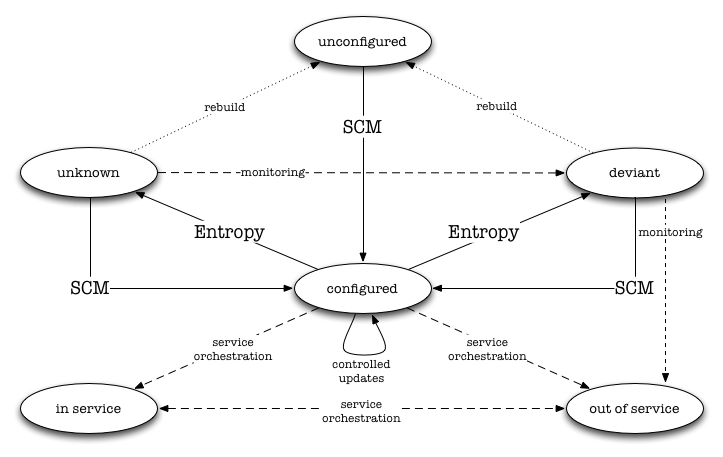
\includegraphics[width=0.95\textwidth]{07/pics/host-states}
		\caption[Host States in Configuration Management]{
			Different states a host may be in.  The CM tries to
			counter the effects of Entropy, while Service
			Orchestration controls e.g. whether a host takes
			traffic.  Monitoring of the systems may allow us
			to discover an ``unknown'' state or trigger a
			removal from service, while rebuilding a host
			allows us to ``start from scratch''.
			\label{fig:configuration-management:host-states}}
\end{figure}


\subsubsection*{Unconfigured}

A host in this state does not have a CM system
installed or the installed CM has never run.  The most
common example of hosts in this state is new hardware
that does not yet have an OS installed. Large
environments often have pools of new hardware
delivered, racked, and set up in their data center,
awaiting allocation.  Such systems are frequently in
this {\em unconfigured} state.

\subsubsection*{Configured} The CM has run
successfully and applied all required changes for the
given system.  All required packages are installed,
configured properly, and all services on the host are
running.  The system is ready for production.

\subsubsection*{In Service}  The host has been put
into production.  That is, it accepts traffic,
provides the service for which it was configured, and
is relied upon; it is in active use.  Technically
speaking, this is a subcategory of the ``configured''
state; a host may be put into service by other systems
than the CM -- we mentioned the concept of ``Service
Orchestration\index{Service Orchestration} -- but only
a ``configured'' host may enter this state.

\subsubsection*{Out of Service} The system has
explicitly been taken out of service; it is no longer
serving production traffic.  Unlike the remaining
states, this is a well-defined and known state.  The
CM is running and may even have placed the system into
this state as a reaction to a system or network
failure, possibly one outside of this host.  That is,
this state is also a subcategory of the ``configured''
state.  Once again, the host may be taken out of
service by another system than the CM.

\subsubsection*{Deviant}  The host is no longer in the
desired configuration state.  Entropy has taken its
toll: changes made to the system either manually or as
a side-effect of the traffic it takes, from individual
users or possibly even through a mistake in the CM
state model itself have caused a faulty configuration.
In this case, the configuration management system may
need to revert or otherwise correct these changes to
revert to the previous state.  Storing the rules for
the CM in a Version Control System makes such a ``roll
back'' easier.

\subsubsection*{Unknown} The CM may have stopped
running on the host or may erroneously be applying the
wrong configuration.  The host may have been shut
down, the network disconnected, an intruder may have
taken over control, or rats may have gnawed through
the power cable.  We simply don't know.  What's worse,
we may not even know that this host is in an unknown
state!  Not all failures are immediately obvious.  \\

Describing a service in detail, as we discussed
earlier in this chapter, and then applying the
required changes to a new host covers the steps to get
a system from the ``unconfigured'' state towards ``in
service''.  This involves a set of well-defined steps,
and the system remains in equally well-defined and
known states.

Much more challenging for both the CM as well as the
system administrators in charge are the prevention and
detection of the last two states, ``deviant'' and
``unknown''.  In order to recover and return the
system back to production, the software needs to be
able to identify error conditions and determine the
steps to correct them.  Automatic recovery from
certain failure scenarios is possible, and in fact
what we wish for our CM to provide.  However, most
software solutions can only handle previously defined
error scenarios; the nature of our systems inevitably
leads to unexpected failure modes.  Being able to {\em
detect} such deviant states is by itself a huge win,
as we can move from here into the much preferred ``out
of service'' state before resolving the root cause and
finally returning the host back into production.  In
some cases it may be easier and/or faster to reinstall
the host from scratch to bring it into a compliant
state.


\subsection{Sets}
\label{configuration-management:states-sets:sets}

Running any CM requires system administrators to
create and maintain a complex model of how services
are defined, what changes are required to enable or
disable a given component, and to keep track of all of
your systems in different environments with different
requirements.  The key to solving this puzzle is to
{\em simplify}: we take a step back and attempt to
identify the essential logical components of the
system.

In the previous section we have classified the
different {\em states} that our systems may be in, and
we have said that the role of a CM is the assertion of
a given state. But before we can express the changes
required to bring a host into a given state, we need
to have defined the role of each system.

%Enter Set theory.  Set theory is a wonderful thing.
%It allows us to completely abstract the functional
%requirements of configuration management into a
%well-understood model that is easy to follow.  Set
%theory allows us to group arbitrary resources and
%give each group a name.  With enough such carefully
%defined sets, we can describe a state model and apply
%it to our infrastructure.  Set theory resides at the
%core of configuration management. \\

Different CMs use different terms in their application
of several concepts that we borrow from Set Theory:
each solution allows for the grouping of certain
resources that can be combined using unions,
intersections, set differences, etc.  For example, sets of
changes or service definitions may be called
``manifests'', ``promises'', or ``recipes'', while
sets of hosts may be referred to as ``roles'', ``node
groups'', or they may be defined through the use of
``attributes'' or ``tags''.

I've found it useful to remember the visual
description of defining these sets as ``drawing
circles around things'': this is quite literally what
developers and system administrators often end up
doing on their whiteboards.  Looking at these
whiteboards or state diagrams immediately conjures the
Venn Diagram, an easy way for us to visualize
relationships between different groups.

As we define services as a set of changes, or hosts as
being grouped together by certain attributes, we can
build an inheritance model using further and further
abstraction of common properties into subsets.  By
performing set operations such as unions,
intersections and set differences, we gain significant
flexibility in determining common and service specific
definitions.

Let us take a look at the different kinds of resources we might draw
circles around:

\subsubsection*{Sets of changes}

Moving beyond maintenance of a few individual hosts,
we realize that changes made on our systems fall,
broadly speaking, into two categories: those that need
to be applied to {\em all} systems\footnote{Ok, we
are cheating a bit here: there rarely are properties
applying to absolutely {\em all} your systems.  In
System Administration in large scale environments,
exceptions are the single universal rule.} (as might
be the case illustrated by our \gls{ldap} Client
Configuration example from Section
\ref{configuration-management:defining-services:ldap-client}),
and those that need to be applied to only a {\em
subset} of systems, possibly a subset of one.  This
realization is fundamental: we begin to view system
configuration no longer as a task performed on an
individual host, but as {\em defining the changes}
that may need to be applied.

In addition, there are changes that are made to all
system {\em in exactly the same way} (e.g., the
{\tt /etc/sshd\_config} file is updated on all hosts to
disable {\tt PasswordAuthentication}) as well as
changes that are made taking specific properties of
the target environment into account (e.g. the use of a
different default route or DNS server depending on the
network the system is in).  The astute reader will
recognize parallels to the four classes of data we
identified earlier: ``static'', ``variable'',
``shareable'' and ``unshareable'' (compare Table
\ref{table:software-installation:shareable-variable}).

It is important to be consistent in the application of
this model:  even a single service running on a single
host should be well-defined and explicitly described
as such a set -- a set of one.  This allows us to
easily recreate the service in case of emergency, when
more resources are added, or when an additional
instance of the service is created, for example in a
new data center.

Figure
\ref{fig:configuration-management:change-states} shows
how different change sets can be combined via an
inheritance model to help define more complex
services.

\begin{figure}[!ht]
	\centering
	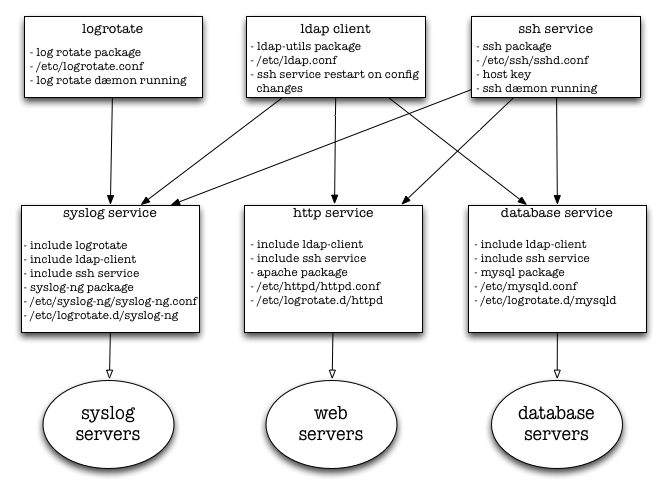
\includegraphics[width=0.80\textwidth]{07/pics/change-sets}
		\caption[Sets of changes applied to sets of hosts]{
			An illustration of how abstract
			change sets help define different services. Common
			modules are included in more complex definitions
			before being applied to groups of hosts.  Some
			``base'' modules (ssh and ldap in this example)
			are included on all hosts.
			\label{fig:configuration-management:change-states}}
\end{figure}

\subsubsection*{Sets of hosts}

Any host may, at any point in time, perform multiple
roles, offer multiple services, or meet multiple
requirements.  Grouping hosts according to their
properties, attributes, or functionality makes it
possible to apply the previously identified sets of
changes.  But groups of hosts are not only defined by
the services they provide; you can also categorize
hosts by different criteria even within a single
service definition.  It is common (and good practice)
to have for each service a small number of hosts --
some of which do not take any production traffic -- on
which to test any changes that we plan on rolling out.
Many organizations use the terms ``dev''
(development), ``qa'' (quality assurance),
``testing'', ``staging'' or ``canary'', and ``prod''
(production) for the different stages of software
development.  Likewise, it may be useful to group
hosts by geographical location to allow for a
carefully staged deployment on a global scale.

Software deployment -- an inherently risky business,
as we are willfully introducing entropy into a running
and stable system -- can thus be carefully
orchestrated through the use of a CM and clearly
defined roles.

In fact, CMs themselves usually allow you to {\em
branch} your changes in the same way that a software
development project may track different development
efforts before merging changes back into the main
line.  In order to take advantage of this approach,
divide your hosts into sets that are on a different
branch: a relativey small number of hosts would
receive all changes immediately, allowing the system
administrators to rapidly test all their changes; a
larger host sample (ideally including a cross section
of all possible host group definitions) should follow
the ``staging'' branch to which changes which need to
be tested would be deployed.  All remaining hosts
track the ``stable'' or ``production'' branch,
receiving changes only after they have gone through
the previous stages and found to be without errors.

See Section
\ref{configuration-management:fighting-entropy:deployment-roles}
for a more detailed description of this approach.

\subsubsection*{Sets of users}

Finally, account management is perhaps the most
obvious application of the principles of set theory
within configuration management.

As noted in Section \ref{multi-user:groups}, user
accounts may be grouped together by their required
access privileges.  Regardless of whether user
accounts are managed centrally via a directory service
or whether individual accounts are explicitly created
on each system, the decision to grant access is based
on a user's group membership ;  user groups are then
mapped to different sets of hosts as previously
illustrated in Figure
\ref{fig:multi-user:user-mappings}.

Note that different users can be simultaneously
members of multiple groups.  In our previous example,
we showed how users in the {\tt wheel} group were
given full {\tt sudo(1)} privileges on all hosts,
while members of the {\tt dev} group might only get
user level access to a small subset of all hosts.
These mappings are non-exclusive: a user may well be
in both the {\tt dev} and the {\tt wheel} groups at
the same time.


\section{Fighting entropy}
\label{configuration-management:fighting-entropy}

Configuration management asserts state.  That is, we
try to keep a system from deteriorating into an
undefined state and to (re-)establish more order.  We
continuously fight entropy.  But we are also
introducing change, and the changes we apply may have
side-effects.  CMs have the potential to completely
bring down an entire infrastructure if the wrong kinds
of changes are introduced.  It is therefore important
to look at a few safeguards and techniques that allow
us to prevent such disaster scenarios.

\subsection{Deployment roles}
\label{configuration-management:fighting-entropy:deployment-roles}

Managing infrastructure code, as it turns out, is not
very different from traditional software development.
The final product needs to be tested before it is
shipped to the customers.  In the context of
configuration management, this might be a service
definition that has to be verified to not
inadvertently break the systems on which is should be
deployed, including new releases of the service
software.

As a result of this similarity, we usually employ
similar strategies and create development, test, and
pre-production environments on which to iterate
through a series of assertions to ensure the
correctness of the installation and configuration.  In
the previous section we already mentioned the grouping
of hosts into these conceptual roles -- and the number
of stages you require a change to propagate through
before it reaches production may depend on the size of
your environment -- but in general, it is a good idea
to have the configuration management development
process to include the following deployment roles.  As
you read through the description of these roles,
reference Figure
\ref{fig:configuration-management:host-sets} for an
illustration.

\begin{figure}[!t]
	\centering
	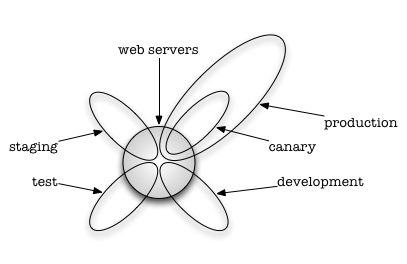
\includegraphics[width=0.65\textwidth]{07/pics/host-sets}
		\caption[Host Deployment Roles as Sets]{An illustration of
			the different deployment roles a host may be in.
			Of all hosts in the ``web server'' group, some are
			in the ``development'' environment, some are in the
			``test'' and ``staging'' environments, and some
			are serving production traffic.  Of those, a small
			subset performs the role of the ``canary''.
			\label{fig:configuration-management:host-sets}}
\end{figure}

\subsubsection*{Development}

These hosts serve as the playground where all
prototypes are initially set up as proofs of concept
before being properly packaged and turned into a
defined service.  All new changes are initially
developed and tested in this environment.  Hosts in
this role are often in a state of flux, and it is not
uncommon for a system administrator to break a service
in the process of testing a new configuration
management module.  For this reason, these systems do
not serve production traffic.

\subsubsection*{Test}

A small number of hosts on which to perform end-to-end
tests after initial development make up the test
environment.  Once we have defined a new service,
created a new package, or made any other changes to
our CM, we let them be applied in this environment.
The most important difference to the ``development''
environment is that {\em we do not perform any manual
changes here}: everything goes through the full
configuration management cycle.  This allows us to
make sure that the module we put together does in fact
include all required changes, can be applied by the
configuration management software, and does not cause
any obvious problems.

In a heterogenous environment it is important to ensure that all major
operating system versions are represented in this group.

\subsubsection*{Pre-Production}

Once testing has determined that the changes we plan
to roll out do indeed yield the desired state, we can
push them into the pre-production environment,
sometimes referred to as ``staging''.  This group
consists of a representative sample of all production
serving hosts, including different hardware
configurations and different operating systems.  For
each major service, a sample of hosts are placed into
this role to ensure compatibility of any new changes
within the given software stack.

Systems in this role do not usually take full
production traffic, but may be used internally to test
your products.  In some environments, a small
percentage of actual production traffic is shifted to
these systems to ensure that all crucial code paths
that might be encountered once the change is deployed
are executed.

Often times we define automated checks and tests that
run against these hosts to ensure no unexpected side
effects were introduced by the changes we made.

\subsubsection*{Production} All hosts serving
production traffic or providing a crucial (possibly
internal only) service.  Any changes made here should
have gone through the previous stages, and in some
cases may require explicit ``change
management\index{change management}'' practices,
including advance notification of all stakeholders,
service owners, and customers.

Since this group of systems can range in size from
only a handful of hosts (for a particular service) to
literally hundreds of thousands of machines (providing
multiple services), deployment of any changes is
inherently risky and needs to be coordinated
carefully.  Especially in very large environments
these changes are often deployed in a staged manner:
starting with a small number of machines the
percentage of all hosts that will receive the change
is slowly ramped up.

\subsubsection*{Canary} Sometimes it is difficult to
account for all eventualities, and experience has
shown that some errors cannot (easily) be reproduced
or triggered in a controlled staging environment.
This is largely due to the fact that actual production
traffic is so difficult to simulate.  Hence, it may be
a good idea to create a so-called ``canary'' role as a
special method of detecting possible errors in your
configuration:  individual hosts that are part of the
actual production environment and that do take
production traffic will get code deployments earlier
than the bulk of the production hosts.  This way,
errors can be detected before they might be deployed
everywhere else.  Like the canary in the coal mine,
these hosts serve as an early warning system for
potentially dangerous changes.

\begin{sidenote}
{\bf Security Roles} \\

Please note that the definitions given here are also
helpful in deciding access control as well as traffic
flow from a security perspective.  For example, hosts
in a {\em development} role may be accessed by all
developers, while production systems may not.
Similarly, traffic may be allowed from hosts in the
``test'' role to other hosts in the same role only,
but access of production data may be restricted to
production systems only. \\ [10pt]

Even though there is a certain overlap in defining
deployment roles and in defining roles related to
security, they are not always congruent.  While access
restrictions may be derived from the deployment model,
finer grained control and additional restrictions or
definitions are often necessary.  Nevertheless, the
model of {\em sets} applies here as well.  Only this
time, we are, for example, drawing circles around
host- and network based \gls{acl}\index{Access Control
Lists} and intersecting these security roles with
host- and user groups.

\end{sidenote}


\subsection{Idempotence and Convergence}
\label{configuration-management:fighting-entropy:idempotence-convergence}
\index{Idempotence}
\index{Convergence}

Configuration management asserts state.  To this end,
it must reliably produce a defined state without
side-effects and needs to be able to run under
different circumstances, yet yield the same outcome.
If you run your CM on an unconfigured system, it will
produce the same end-result as if you run it
repeatedly, over and over, in its final, configured
state.

Operations that can be performed multiple times yet
always produce the same result are called {\em
idempotent}.  To illustrate, unary mathematical
operations are idempotent if the following definition
holds:

\begin{displaymath}
f(f(x)) \equiv f(x)
\end{displaymath}

That is, a function applied twice to any value will
produce the same result as if applied only once.  A
common example here is taking the absolute value of
$x$:

\begin{displaymath}
| |-1| | \equiv |-1|
\end{displaymath}

%For binary operations, the definitions get a bit more
%complicated: an idempotent function applied to two
%equal values will return that value (e.g. $max(x,x)
%\equiv x$), but for other operations there may exist
%only some elements that satisfy idempotence:
%multiplication by $0$ or $1$, or division by $1$, are
%examples of idempotent elements on binary operations:
%no matter how often you repeat this operation, the
%end result will remain identical.

How does this property translate into practical
applications within the scope of configuration
management?  As we are moving the system from one
state to another, we are applying certain changes.
Executing these steps must not yield different results
depending on the previous system state.  Reviewing the
required capabilities we identified as CM requirements
in Section
\ref{configuration-management:defining-services:requirements}
-- software installation, service management, file
permissions and ownerships, installation of static
files, generation of host-specific data, and command
execution -- we find that each may or may not be
implemented in a manner that satisfies this
requirement.  As one example, assertion of an existing
file's ownership and permissions, is an inherently
idempotent operation: no matter how often you execute
these commands, and no matter what the permissions and
ownership on the file were before, the end result will
be the same.

Other typical tasks within configuration management
are not quite as obviously idempotent, and some --
updating an existing file on a host with parameters
determined at runtime, for example -- may in fact
not be.  For any command executed within a
configuration management system, you can ask yourself
the question of whether or not the outcome will be the
same if you either run the command under different
circumstances, or if you repeat the command over and
over.  See Listing \ref{code:cm:idempotence} for a few
trivial examples.  Note that sometimes a command may
behave idempotently only if a special flag is given, and
that under some circumstances the only thing that
makes a command {\em not} idempotent may be the exit
status.  (We will revisit the importance of
idempotence within the context of building scalable
tools again in Chapter
\ref{chap:building-scalable-tools}.)

\begin{lstlisting}[basicstyle=\scriptsize,float,label=code:cm:idempotence,caption={Idempotent and non-idempotent commands.}]
$ cd etc                                            # not idempotent
$ rm resolv.conf                                    # idempotent
$ echo "nameserver 192.168.0.1" > resolv.conf       # idempotent
$ echo "nameserver 192.168.0.2" >> resolv.conf      # not idempotent
$ chown root:wheel resolv.conf                      # idempotent
$ chmod 0644 resolv.conf                            # idempotent
\end{lstlisting}

In many cases the CM may aid in defining actions in
such a manner as to preserve idempotence -- {\em
CFEngine}, for example, explicitly discourages the use
of free shell commands and leads the user to abstract
their requirements into so-called
``promises''\cite{configuration-management:cfengine-manual}
-- but in the end it is up to the system administrator
to carefully evaluate the service definitions and
change sets she creates and applies to ensure that no
side-effects are possible.

Idempotence goes hand in hand with the philosophy of
asserting state, rather than making changes.  Writing
system tools and defining changes that are idempotent
takes great care and consideration, especially when
one considers the possibility of simultaneous
execution of commands or programs outside of our
control.  The time and effort spent on identifying
these and creating a tool that can cope with these
factors yield significant benefits: System stability
increases as we are able to reliably repeat the same
commands without fear or unwanted side-effects.  \\

It is important to note that idempotence does {\em
not} imply that an operation is {\em only} performed
when it is necessary, only that the {\em outcome} will
remain the same.  That is, idempotence does not
guarantee efficiency nor necessarily continuous
service availability.  Consider two systems, one brand
new and unconfigured, one already in a desired state,
i.e. a production service.  In order to get the first
system into the state of the second system, the CM
needs to make a lot of rather intrusive changes:
software packages have to be installed, configuration
files updated, and the host may need to be rebooted,
possibly multiple times.  Performing all of these
steps again when the end state would be the same as
the current state seems like a bad idea.  At best,
we'd be wasting CPU cycles; at worst, we'd introduce
temporary instability or service downtime.

This is where the concept of {\em
convergence}\index{Convergence} comes into play:  A
configuration management system should only perform
those operations and apply only those changes that are
necessary.  Idempotence and Convergence are easily
conflated, and within a CM, both are desired
properties.  But it is important to be aware of the
difference:

Consider the \verb+chown(8)+ and \verb+chmod(1)+
example code from Listing \ref{code:cm:idempotence}.
Despite being idempotent, running the commands may not
be necessary at all if the permissions and ownerships
are already as desired.  That is, the configuration
management system could first test for the desired
end-state, and then only execute the steps missing.
In this particular example, the difference is
negligible, but the practice of checking whether
commands actually need to be executed becomes more
important when we consider how our system may assert
the presence of a certain software package.

That is, if a package of the required version is
already installed, the CM (possibly by way of the
package manager it invokes) will likely perform a
no-op instead of fetching the same package and
re-installing it.  This is {\em not} the same as
performing the installation again:  for example, all
too frequently poorly packaged software may overwrite
your carefully tuned existing configuration file with
a new template or example file.  A good package
manager, and a carefully written package, may be able
to prevent this from happening, but you cannot always
rely on this.

Different CMs provide different features, and being
able to use them all to your advantage requires
practice.  In some systems, the responsibility of
defining convergent operations is pushed on the system
administrator; other CMs go to great lengths to avoid
unnecessary changes.  Idempotence is crucial for all
operations within a CM, but allowing the system to
reach the end state in a convergent manner improves
stability and reduces the possibility for service
interruptions on the way from state A to state B.
Both principles are often fully understood and
appreciated only after a lot of practical experience
and a perhaps a few ``interesting'' error scenarios,
but try to keep them in mind as you develop and deploy
your CM solution.

\subsection{Quis custodiet ipsos custodes?}
\label{configuration-management:quis-custodiet}

The latin phrase ``{\em Quis custodiet ipsos
custodes?}'' -- translated: ``Who will guard the
guards themselves?'' -- expresses a fundamental
dilemma we encounter when we give full control to any
person, government body or, in our case, a piece of
software.  That is, configuration management asserts
state, but what ensures that the configuration
management system functions properly?

In fact, CM systems usually control {\em themselves}.
After all, configuration management is a software
service just like any other, and needs to be
controlled and monitored the same way.  This, however,
introduces a rather significant risk factor, as
changes made to the CM itself have the ability to
either wreak havoc across the entire infrastructure or
to simply halt any progress if it breaks down.

For this reason, it is important to put in place
safeguards and practices to reduce the probability of
such errors.  The risk of potential disaster is one of
the side effects of a high degree of automation.  We
will discuss this and a number of possible risk
mitigating techniques in detail in Chapter
\ref{chap:automation}.

\section{Even more formal process definitions}
\label{configuration-management:formal}

Today's CM systems exhibit a noticable overlap with
concepts discussed in the \gls{itil}\index{Information
Technology Infrastructure
Library}\cite{configuration-management:itil}, a set of
practices underlying the first international standard
for IT Service Management, ISO/IEC 20000\index{ISO/IEC
20000}.  As a formalized standard trying to cover
generally applicable practices, these documents offer
a far from thrilling reading experience and have seen
limited voluntary adoption in the private sector.  The
main criticisms are similar to those applied to
similar standard documents and regulations (such as
the notorious \gls{pcidss}\index{PCI DSS}): good
intentions and sound general advice is lost amidst
lenghty rationale and overly bureaucratic and much too
broad definitions.

As perhaps a form of social commentary, one might be
further inclined to seek parallels between modern CM
systems and a general Silicon Valley startup culture
of rapid invention and quick iteration versus an as
``old and stuffy'' dismissed IT process represented by
the formality of \gls{itil}.  As so often, software
systems reflect the organizational and cultural
hierarchies under which they are
developed\footnote{See ``Conway's Law'', derived from
\cite{configuration-management:conways-law}\index[names]{Conway,
Melvin E.}.}; most System Administrators with
sufficient experience will find some humor in the fact
that nevertheless, even these different methodologies
become eventually convergent.

That is, despite being easily dismissed as not
flexible enough for practical application, many of the
recommendations or best practices outlined in ITIL do
underly or correlate to the operations of modern CMs.
For example, large scale configuration management has
evolved to effectively implement or require a
repository of all information about the various
systems in an organization, the Configuration
Management Database\index{Configuration Management
Database} (or CMDB).  When you read up on this topic,
you will hopefully be able to relate those documents
to a number of concepts discussed here.




\section{Summary}
\label{configuration-management:summary}

We have covered a lot of ground in this chapter, much
of it theoretical.  The examples shown were taken from
some of the more popular configuration management solutions
currently in use: CFEngine, Chef, and Puppet.  All
three implement their own Domain Specific Language,
with striking similarities amongst them.

We identified as one crucial concept in configuration
management the idea that services are abstracted from
the hosts that provide them.  This abstraction allows
us to define not individual changes, but rather
self-contained change sets describing what is required
to provide a given functionality.  These change sets,
in turn, can be applied to groups of hosts; with those
sufficiently abstracted and clearly defined, we are
able to combine attributes of host groups and describe
its members' final state using set operations.  Much
like on a white board or the proverbial paper napkin
in a restaurant, we draw circles around things.
Giving those circles descriptive names, configuration
management then becomes a question of creating unions
or intersections of service descriptions with host
collections.

Using this model, we determined that configuration
management is really not about {\em applying changes},
but about {\em asserting state}, ensuring that a host
meets a certain set of criteria.  We have looked at
the functional requirements any CM needs to provide in
order to yield a desired state as well as the
essential concepts of idempotence and convergence: all
changes we make must have well-defined and predictable
outcomes that do not change if applied repeatedly; at
the same time, we only want to perform those changes
that are necessary.

When building our infrastructure we face a choice
between a custom, home-grown system that integrates
perfectly with other system components, and deploying
an ``Off The Shelf'' solution.  Many commercial
products exist that promise to manage all of your
systems with ease.  Some of them offer free versions;
some systems are available as open source software,
while others are closed.

Knowing our infrastructure needs inside and out, we
often fall into the trap of writing our own solutions.
In small environments, the benefits of a complex
product do not seem worth the cost of adapting our
infrastructure to abide by the product's configuration
model.  It is for this reason that every growing
company inevitably undergoes a phase during which
large parts of the initial infrastructure are ripped
out and replaced by more scalable solutions --
including a mature configuration management system.

In very large environments, on the other hand, our
requirements are so unique as to not likely to be
matched trivially by any available solution; we will
need to write a significant amount of ``glue'' code
around the product anyway -- why not just implement
our own system?  But therein lies a frequent fallacy:
as any software engineer knows, the best code is the
one we do not have to write ourselves.

Fortunately, development on a number of flexible CMs
has yielded several viable solutions for almost any
scale.  A small environment benefits from the rigorous
structure imposed by a mature configuration management
system able to grow with the infrastructure; in large
environments, it is useful to be able to rely on a
proven technology and focus on the end point
integration with other systems.  \\

The area of configuration management has become one of
the most important fields in large scale system
administration and has opened up room for a lot of
interesting research.  As this chapter hints at, there is
significant overlap between configuration management,
software provisioning\index{Provisioning}, and the
many related tasks in ensuring reliable service
availability.  All of these moving parts are sometimes
referred to as ``Service Orchestration''\index{Service
Orchestration}, by now its own field of research
covering the theory of how complex systems fail, in
how far we can achieve automatic recovery or guarantee
service availability, and the concept of autonomous
state configuration across large scale deployments
with literally hundreds of thousands of hosts.  See
Figure \ref{fig:configuration-management:cm-overlap}
for an illustration of these relationships.

\begin{figure}[!t]
	\centering
	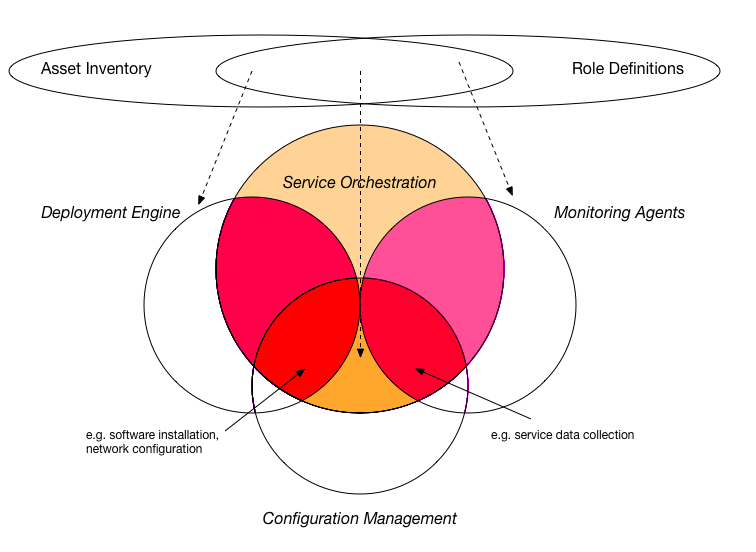
\includegraphics[width=0.65\textwidth]{07/pics/config-management-overlap}
		\caption[Configuration Management Overlap with other systems]{
			Configuration Management overlaps and
			intersects several other areas
			of System Administration, many
			of which depend on a central asset database and
			comprehensive service definitions.
			\label{fig:configuration-management:cm-overlap}}
\end{figure}

As so often, we can only focus on the fundamental
concepts with just enough references to more advanced
topics to entice the reader to continue their
research. We will revisit some of these topics in
section \ref{sec:missing:service-orchestration}, when
we try to catch up on missed topics and tie together
some of our loose ends. \\

Throughout this chapter, we have focused primarily on
configuration management of host-type systems.  But
our infrastructure consists of more than just
``hosts'': we have large amounts of network
equipment as well as a number of appliances that sit
somewhere in between the traditional networking gear
and a ``normal'' host: we have routers and switches,
load balancers and firewalls, storage devices and
intrusion detection systems... the list goes on.  All
of these devices {\em also} require configuration
management, and it is unfortunate that integrating
them into your existing CM is often difficult, if not
impossible.

Our approach to divide resources into grouped sets and
describe changes as service definitions does in fact
translate to non-host systems as well.  All we need is
for a programmatic method to access them -- ideally,
though not necessarily via a programmable interface
such as a well-documented \gls{api} -- and we can add
support for them to our CM.  A positive development in
recent years has lead some of the configuration
management tools we mentioned to now allow you to
manage at least some non-host type systems, even
though we are still a ways from the same level of
control.  \\

The fundamental value configuration management provides as
we move from individual systems to easily replicated
services is perhaps best summarized by this quote:

\begin{quote}
``The test we use when designing infrastructures is "Can I grab a random
machine that's never been backed up and throw it out the tenth-floor
window without losing sysadmin work?" If the answer to this was "yes",
then we knew we were doing things
right.''\cite{configuration-management:traugott}
\end{quote}

Granted, one would hope that people entering your
datacenter and throwing machines out of the window is
not a regular event.  But Murphy's famous
law\index{Murphy's Law} -- commonly cited as ``Anything
that can go wrong, will go wrong.'' -- acts as
viciously, and we must view software failure as the
functional equivalent.  All software has bugs, and it
is only a question of time until your complex service
encounters a fatal error.  Similarly, hardware fails
as well -- and not too infrequently.  This becomes
painfully obvious in very large environments with
hundreds of thousands of machines, as the probability
of encountering a hardware failure increases
proportionally to the number of hosts in service.
``One in a million is next
Tuesday.''\cite{configuration-management:next-tuesday}

With properly defined services, correctly grouped
hosts, and a well running CM individual hosts do
become expendable.  Any system-, software-, or
hardware failure has significantly reduced impact on
our overall service availability.  In other words:
configuration management lies at the heart of any
well-managed infrastructure and makes large scale
deployments ultimately maintainable.

\vfill
\pagebreak

\chapter*{Problems and Exercises}
\addcontentsline{toc}{chapter}{Problems and Exercises}
\section*{Problems}
\addcontentsline{toc}{section}{Problems}

\begin{enumerate}

\item

Review your own environment, your infrastructure, and
your essential services.  Do you think they could be
rebuilt from scratch?  With how much effort?  Which
components seem completely and easily replaceable, and
which would you fear most to lose?

\item

Identify the configuration management system currently
in use on the systems you have access to.  Can you
determine which components or services are controlled
by the CM in question and which resources are not?
Contact your system administrator and ask her about
details.

\item

Review the documentation for one of the popular CMs.
Most of them can quickly and easily be tried out using
just a few virtual machines.  Set up a CM and try to
define a simple service.  How does this system
implement the features and concepts we discussed?

\item

Pick a popular service provided in your environment --
for example a DNS-, web- or file server -- and create
a complete service definition for it.  Make sure to
identify the smaller required modules this service
relies on.  How far does it make sense to abstract the
individual components?

\item

When deploying a new service, identify the different
categories into which each step falls.  Is software
installation sufficiently covered by executing the
right commands using your package manager?  Do
additional files need to be created or existing
configuration files modified?  Does the configuration
file differ from host to host within a service group?

\item

Review how your existing package management system
handles reinstallation of a package of either the same
or a different version.  How are configuration files
handled?  Are these actions idempotent?

\item

Consider the agent bundle shown in Listing
\ref{code:cm:cfengine:dynamic-restart}.  What kind of
parameters in the {\tt sshd\_config} file would you
expect to be expanded when this code is executed?
Using CFEngine's online documentation, create a
suitable template.

\item
Review the commands shown in Listing
\ref{code:cm:idempotence}.  Do you agree with their
classification as being idempotent or not?  Try to
argue for or against their classification.

\item
Consider the command ``{\tt mv this there}'' -- under
what circumstances is this particular invocation
idempotent?  Is it ever?  What, if any, checks or
changes can you add to a script that includes this
command to ensure the outcome {\em is} idempotent?

\item
A common test of a new CM consists of updating the
{\tt /etc/motd} file with information from the running
host.  This operation incurs a very small risk, as no
application relies on this file, yet it can easily
show that the system is running and operating
properly.

Create a script or command to update the {\tt
/etc/motd} file on a system to include the hostname of
the system, the time since the host was last rebooted,
and the time this script was last executed.  Can you
translate this script into a template in the \gls{dsl}
of your configuration management system?

\item
Review the different states your systems may go
through.  How do you currently define a properly
operating host?  How would you go about identifying a
{\em deviant} host?

\item
Every System Administrator has a virtual tool chest
full of scripts, commands, and utilities used during
the configuration and maintenance of their systems.
Review your peers' tools as well as your own and
identify in how far they assure {\em idempotence} or
{\em convergence}.  Compare these to the common tools
provided by your Unix systems (such as the scripts
found under {\tt /etc/rc.d} or {\tt /etc/init.d}) or
shipped with a given software package.

\end{enumerate}

\vfill
\pagebreak

\bibliographystyle{plainnat}
\begin{thebibliography}{99}

\bibitem{configuration-management:burgess:cfengine} Mark Burgess, {\em A
Site Configuration Engine}, USENIX Computing systems, Vol8, No. 3, 1995;
on the Internet at 
{\url http://cfengine.com/markburgess/papers/paper1.pdf} (visited February
22, 2013)

\bibitem{configuration-management:nelson-smith:chef} ``An Overview of
Chef'', on the Internet at
{\url http://docs.opscode.com/chef\_overview.html} (visited February 23,
2013)

\bibitem{configuration-management:turnbull:pro-puppet} James Turnbull,
Jeffrey McCune, {\em Pro Puppet}, Apress, 2011

\bibitem{configuration-management:ansible} ``Ansible
Documentation'', on the Internet at
{\url https://docs.ansible.com/} (visited March 18,
2017)

\bibitem{configuration-management:itil} Cabinet Office, {\em ITIL
Service Operation 2011 Edition (Best Management Practices)}, The
Stationery Office, 2011

\bibitem{configuration-management:burgess:immunology} Mark Burgess, {\em
Computer Immunology}, Proceedings of the Twelfth Systems Administration
Conference (LISA 100) Boston, Massachusetts, December 6-11, 1998,
USENIX Association, Berkeley, CA, 1998; on the Internet at
{\url
http://www.usenix.org/event/lisa98/full\_papers/burgess/burgess.pdf}
(visited January 29, 2013)

%\bibitem{configuration-management:set-theory} Georg Cantor, ``\"{U}ber eine
%Eigenschaft des Inbegriffs aller reellen algebraischen Zahlen'', Journal
%f\"{u}r die reine und angewandte Mathematik, 1874; on the Internet at \\
%{\url http://www.digizeitschriften.de/main/dms/img/?PPN=GDZPPN002155583}
%(visited March 10, 2013)

\bibitem{configuration-management:turing-equivalence} Steve Traugott,
Lance Brown, {\em Why Order Matters: Turing Equivalence in Automated
Systems Administration}, Proceedings of the USENIX Large Installation
System Administration conference, Philadelphia, PA Nov 3-8, 2002,
USENIX Association, Berkeley, CA, 2002; on the Internet at
{\url http://www.infrastructures.org/papers/turing/turing.html} (visited
January 29, 2013)

\bibitem{configuration-management:burgess:models-myths} Mark Burgess, {\em
Configuration Management, Models and Myths},  Originally published in
Usenix ;login: 2006-2007; on the Internet at
{\url http://cfengine.com/markburgess/cm.html} (visited January 29, 2013)

\bibitem{configuration-management:brooks-design}Frederick P. Brooks, Jr.,
{\em The Design of Design}, Addison-Wesley Professional, 2010

\bibitem{configuration-management:cfengine-manual} {\em CFEngine
Documentation}, on the Internet at
{\url https://cfengine.com/manuals/}

\bibitem{configuration-management:burgess:rosegarden} Mark Burgess, {\em
Promise you a Rose Garden}, On the Internet at
{\url http://cfengine.com/markburgess/rosegarden.pdf} (visited January 29, 2013)

\bibitem{configuration-management:lueninghoner} Cory Lueninghoner, {\em
Getting Started with Configuration Management}, Originally published in
Usenix ;login: April 2011, Volume 36, Number 2; on the Internet at
{\url https://www.usenix.org/system/files/login/articles/105457-Lueninghoener.pdf}
(visited January 29, 2013)

\bibitem{configuration-management:burgess:testable} Mark Burgess, {\em
Testable System Administration}, in {\em ACM Queue}, January 2011, Vol. 9
No. 1, ACM, New York, NY; on the Internet at
{\url https://queue.acm.org/detail.cfm?id=1937179} (visited January 29, 2013)

\bibitem{configuration:management:couch} Alva Couch, Yzihan Sun, {\em On
the Algebraic Structure of Convergence}, in {\em Proc. 14th IFIP/IEEE
International Workshop on Distributed Systems: Operations and Management},
Heidelberg, Germany, Springer-Verlag, Inc, pp. 28-40

\bibitem{configuration-management:traugott} Steve Traugott, Joel
Huddleston, Joyce Cao Traugott, {\em Best Practices in Automated System
Administration and Infrastructure Architecture: Disaster Recovery}; on the
Internet at
{\url http://www.infrastructures.org/bootstrap/recovery.shtml} (visited March
09, 2013)

\bibitem{configuration-management:conways-law} Melvin
E. Conway, {\em How Do Committees Invent?}, in {\em
Datamation magazine}, April, 1968; on the Internet at
{\url
http://www.melconway.com/Home/pdf/committees.pdf}
(visited April 04, 2017)

\bibitem{configuration-management:next-tuesday} Larry
Osterman, {\em One in a million is next Tuesday},
March 30, 2004; on the Internet at
{\url
http://blogs.msdn.com/b/larryosterman/archive/2004/03/30/104165.aspx} (visited April 04, 2017)

\end{thebibliography}
